\chapter{Introduction to the CS Saucer}
\label{chap:Introduction}
This chapter will provide a background on the chosen experimental surface vessel, CS Saucer (CSS), and its operational environment, the Marine Cybernetics lab (MC-lab).

Initially designed by \citet{idland2015marine}, in collaboration with Ph.D. candidate Andreas Reason Dahl, the CSS is a highly maneuverable drone with a symmetric, circular hull. It was designed this way so behavior would be similar in surge and sway, thus yielding quicker response and maneuverability than a conventional ship model. Modularity was also an essential consideration in the design process, so the vessel uses interchangeable top modules that allow for various payload configurations. \citet{sharoni2016marine}, for example, installed an inverted pendulum, while \citet{ueland} installed a LiDAR-scanner on a separate cover. This modularity was the main draw of the Saucer, as it would make integrating a camera with the already existing lidar relatively easy. 

Recently, the other ships of the cyber fleet, namely the CS Enterprise 1 (CSE1) and the CS Arctic Drillship (CSAD), had their National Instruments (NI) compactRIO embedded computers wholly replaced. The new state-of-the-art system uses a Raspberry Pi (RPi) running a Python and Robot Operating System (ROS) based control system. \citet{idland2015marine} initially implemented the control system of the CSS on a NI LabVIEW platform as well, where the embedded hardware device NI myRIO functioned as the central processing unit. \citet{ueland} and \citet{sharoni2016marine} later replaced this system with a Robot Operating Software (ROS) based solution, running on an RPi 2 as the embedded computer in conjunction with an Arduino as part of their master theses. This provided even more flexibility in development due to the accessibility of ROS-compatible hardware and software.

\begin{figure}[ht]
    \centering
    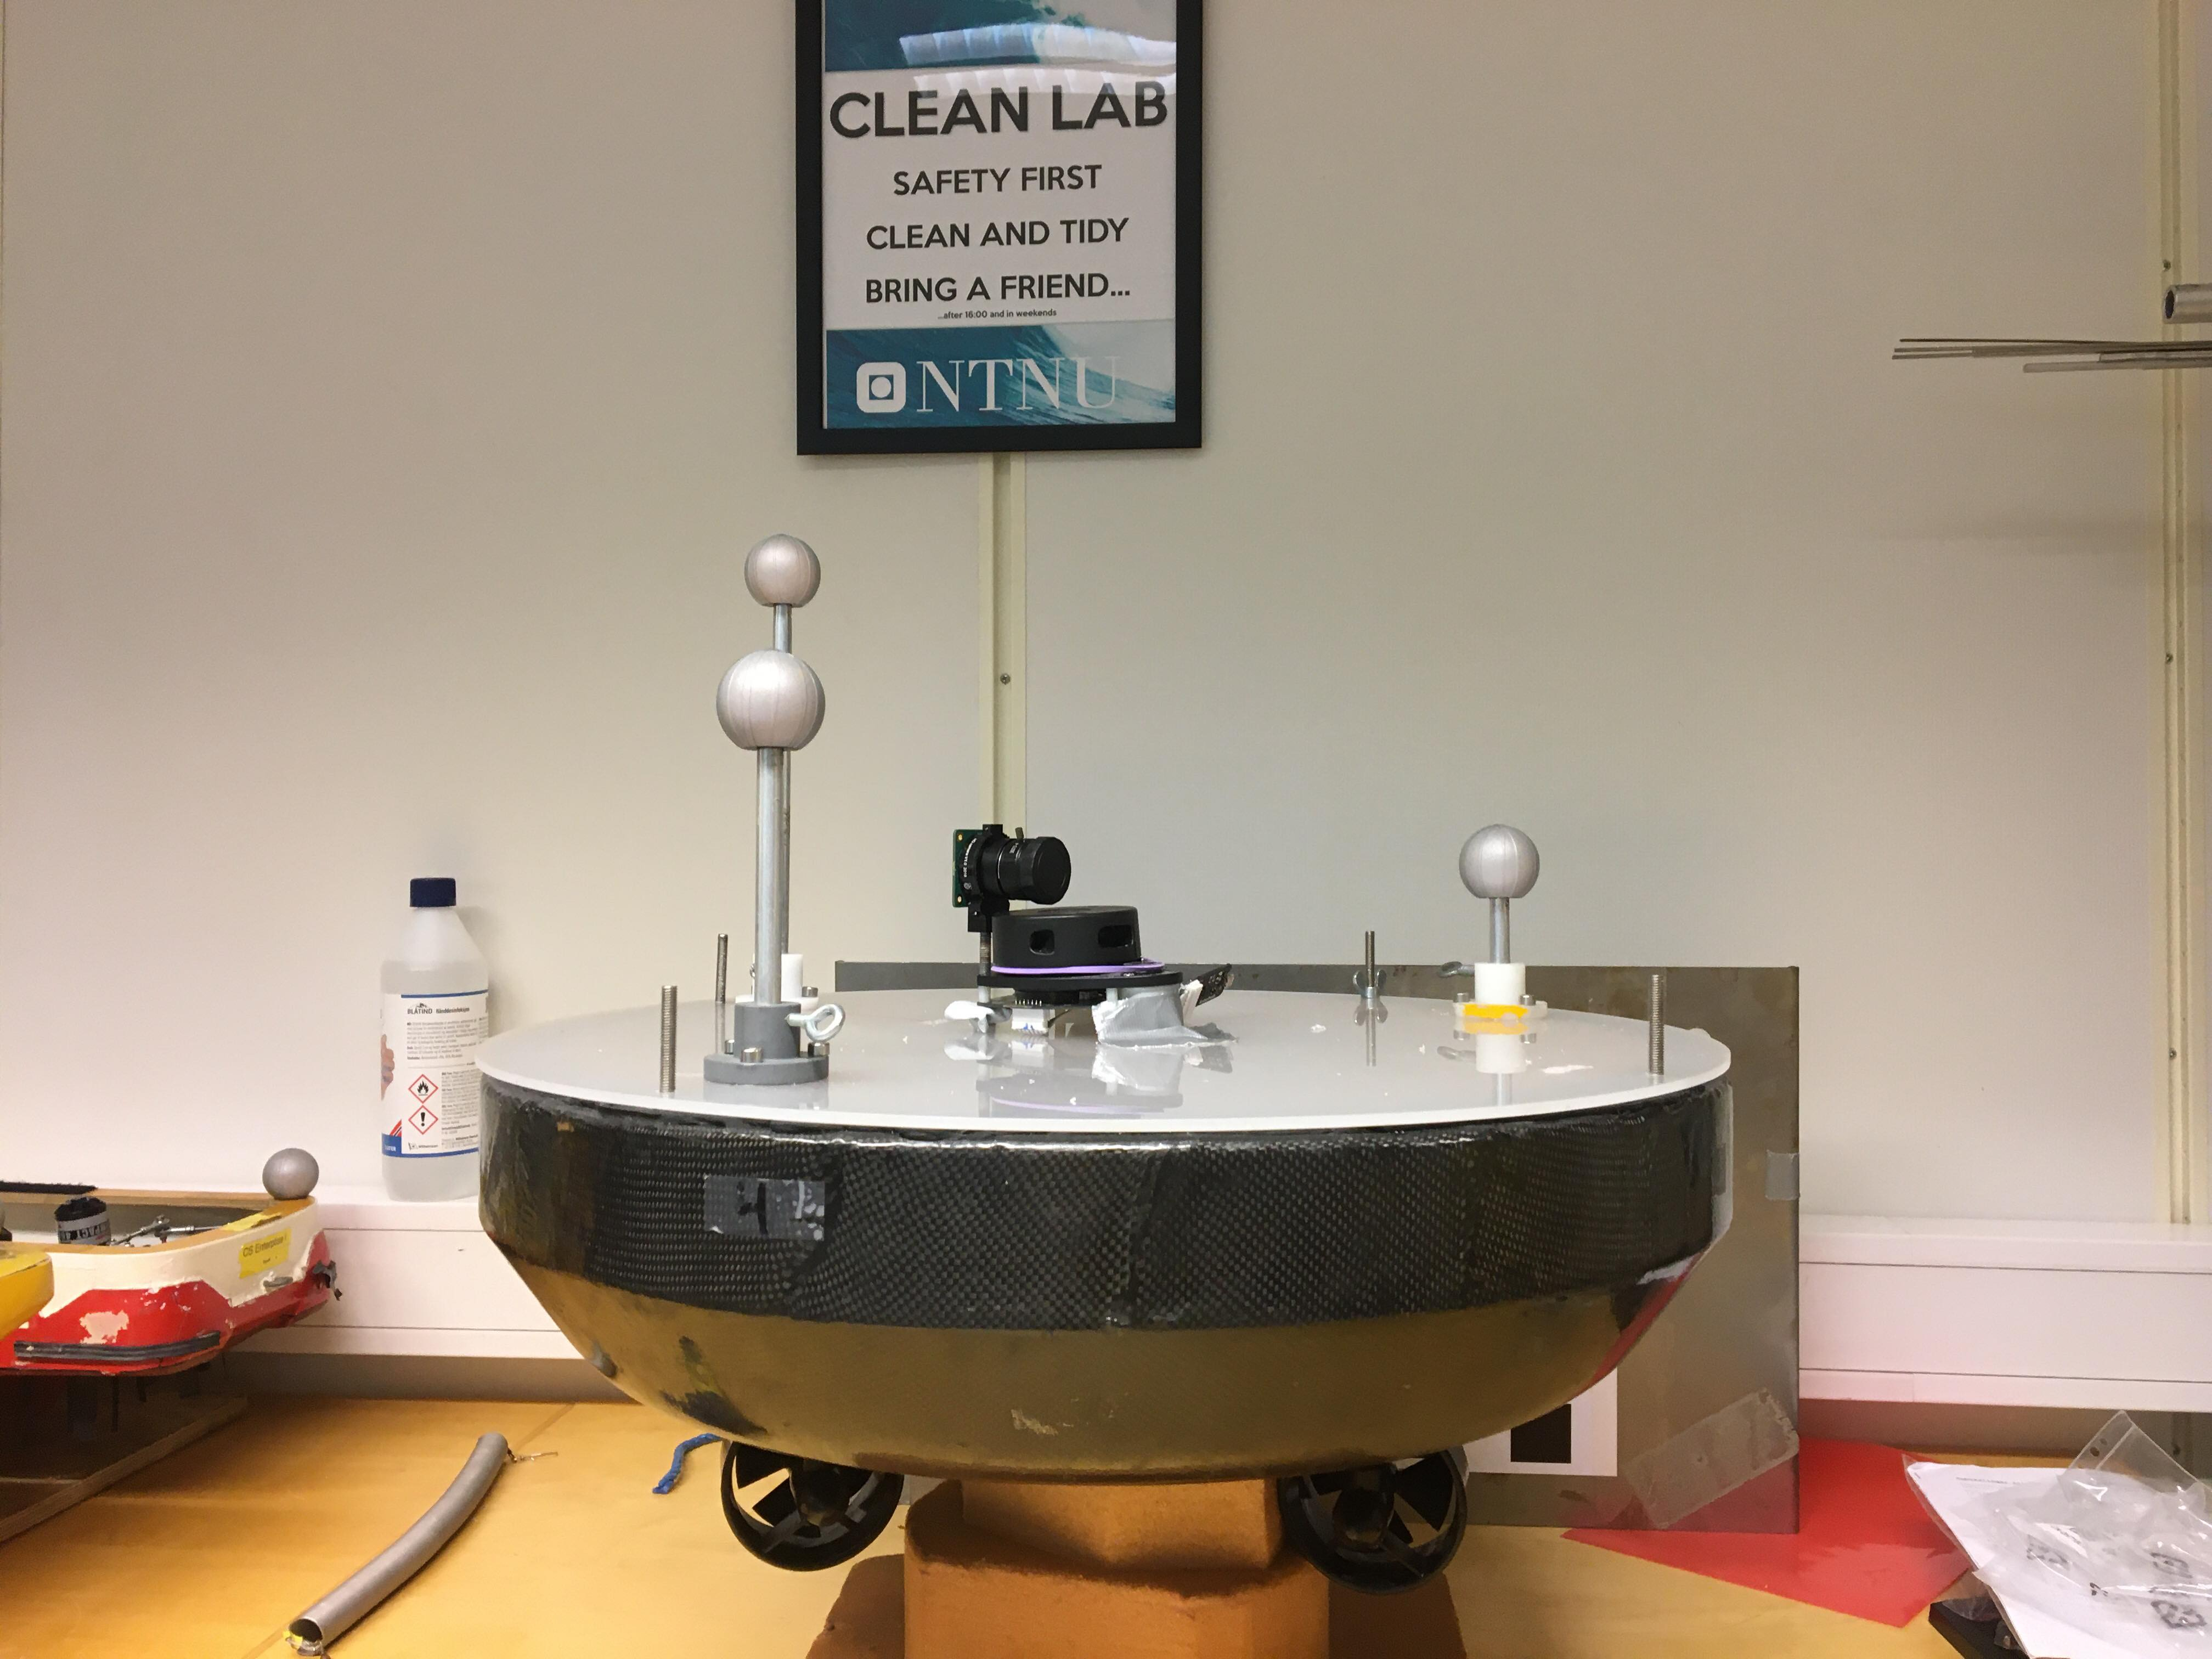
\includegraphics[width=0.8\textwidth]{Images/cssaucer.jpg}
    \caption{The CS Saucer with the latest module installed}
    \label{fig:suacer}
\end{figure}

A final upgrade to the Saucer was conducted as part of \citet{solheim-master}, harmonizing the system with the other vessels. 

\section{Literature}

The development of CSS is a product of much research from several theses, which contain complementary information on the theory applied to the system.

\subsection{Specialization projects and master theses}

\begin{itemize}
    \item Marine Cybernetics Vessel CS Saucer: - Design, construction and control - \citet{idland2015marine}
    \item Marine Inverted Pendulum - \citet{sharoni2016marine}
    \item Marine Autonomous Exploration using a Lidar - \citet{ueland}
    \item Sensor Fusion between camera and lidar for C/S Saucer - \citet{solheim}
    \item Integration between lidar- and camera-based situational awareness and control barrier functions for an autonomous surface vessel - \citet{solheim-master}
\end{itemize}

\section{Technical specification}

As part of the control system upgrade performed in this thesis, several new components were installed on the vessel. \cref{tab:techspec} provides a technical specification of the current state-of-the-art hardware utilized on the vessel. It also includes software utilized during operations. \cref{fig:signal-flow} illustrates the signal and power flow between each hardware component. For a more detailed review of the components, the reader is referred to either \citet{solheim} or \citet{ueland}. Components and software added as part of the control system upgrade are marked with a star ($\star$).

\begin{table}[H]
    \centering
    \begin{tabular*}{\linewidth}{ll}
    \toprule
    \multicolumn{2}{c}{\Large \textbf{Technical Specification}} \\
    \midrule
    \multicolumn{2}{l}{\large \textbf{Software}} \\
    \midrule
    Operating System & Ubuntu 20.04 LTS (Server version)$^\star$ \\
    ROS distrubution & Noetic$^\star$ \\ 
    \midrule
    \multicolumn{2}{l}{\large \textbf{Hardware}} \\
    \midrule
    \multicolumn{1}{l}{\textbf{Component}} &  \multicolumn{1}{l}{\textbf{Description}}\\
    \hline 
    Raspberry Pi 4b$^\star$ & Embedded computer for the vessel. Handles running \\ & ROS-nodes and communication between components \\ & in the system. \\ 
    &\textbf{Processor}: Quad-core Cortex-A72 @ 1.5 GHz.\\ 
    &\textbf{RAM}: 8 GB LPDDR4-3200 SDRAM\\ 
    &\textbf{Power}: 5V via USB-C \\
    \hline 
    Arduino Mega & Embedded circuit board responsible for transmitting \\ & appropriate PWM signals to each component.  \\ & Communicates with the RPi 4b via USB. \\ & Duty cycle between 4.3 and 9.4 \%. \\
    \hline
    Raspberry Pi HQ camera$^\star$ & Camera module \\
    & \textbf{Resolution}: 4056x3040 (12.3 Megapixels) \\
    & \textbf{Framerate}: 30 fps (at highest resolution) \\
    & \textbf{Sensor}: SONY IMX477 \\
    & \textbf{Lens}: 6mm wide angle \\
    \hline
    RPLidar A1 & Low cost $360^\circ$ 2D laser scanner with adjustable \\ & rotation speed. \\ 
    & \textbf{Effective range:} $\SI{12}{m}$ \\
    & \textbf{Sampling rate:}  $\SI{2000}{Hz}$ \\
    & \textbf{Angular resolution:} $\SI{1}{deg}$ \\
    & \textbf{Range accuracy:} $1\%<\SI{3}{m}$, $2\% \in [3, 5] \ m, 2.5\% > \SI{5}{m}$ \\
    \hline
    Torpedo 800 & Motor drive for the three azimuth thrusters. Can spin \\ & the propellers clockwise or counterclockwise. \\
    \hline
    Graupner Schuttel drive unit II & Servo driver to set azimuth angle. Can rotate on the \\ & interval $[-114^\circ, 114^\circ]$. \\
     \hline
    Traxxas LiPo & Three cell, $\SI{11.1}{V}$ lithium polymer battery. Powers \\ 
    & all devices on the vessel. At full charge, either $\SI{640}{mAh}$ \\ & or $\SI{500}{mAh}$, depending on the battery used, it can \\ & power the system for several hours. \\
    \bottomrule
    \end{tabular*}
    \caption{Technical specification for the CSS}
    \label{tab:techspec}
\end{table}

A second computer, referred to as the operator computer, is used together with the embedded computer on the CSS. The primary purpose of the computers is to run the computationally expensive visual detection and fusion nodes. Ideally, the computer should have a GPU to power the CNN, but since the system is designed with low computational availability in mind, a powerful CPU suffices. Therefore, for most of this thesis, a Dell laptop equipped with an 8-core Intel i5 vPro processor was utilized. Like RPi, the computer ran Ubuntu 20.04 LTS and ROS Noetic. 


\begin{figure}[H]
    \centering
    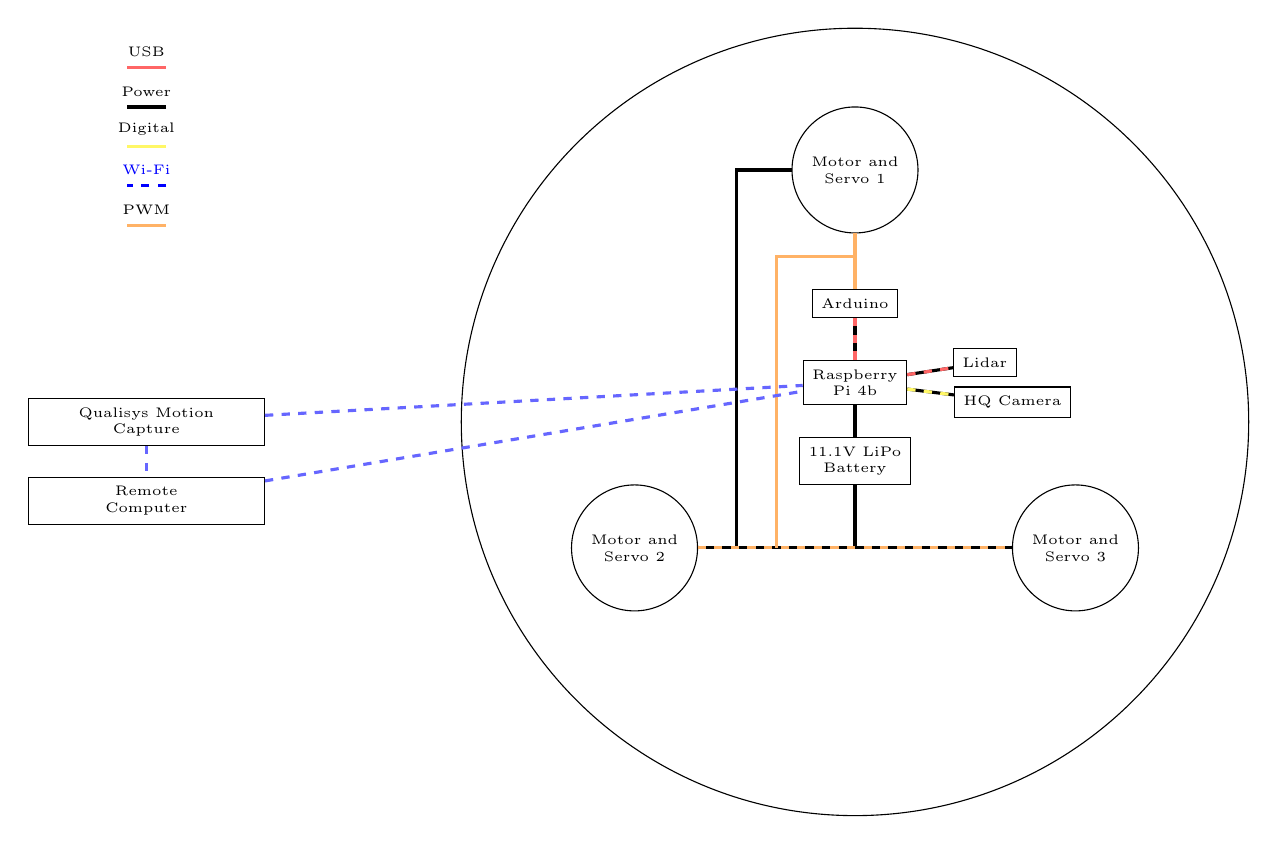
\begin{tikzpicture}
        
        \draw (0, 0) circle(5);
        \draw (0, 3.2) circle(0.8) node[text=black, every text node part/.style={align=center, font=\tiny}] (Motor1) {Motor and \\ Servo 1};
        \draw (2.8, -1.6) circle(0.8) node[text=black, every text node part/.style={align=center, font=\tiny}] (Motor3) {Motor and \\ Servo 3};
        \draw (-2.8, -1.6) circle(0.8) node[text=black, every text node part/.style={align=center,font=\tiny}] (Motor2) { Motor and \\ Servo 2};
        \node at (0, 0.5) [rectangle, draw,  text=black, every text node part/.style={align=center,font=\tiny}] (RPi) {Raspberry \\ Pi 4b};
        \node at (0, 1.5) [rectangle, draw, text=black, every text node part/.style={align=center,font=\tiny}] (Arduino) {Arduino};
        \node at (0, -0.5) [rectangle, draw, text=black, every text node part/.style={align=center,font=\tiny}] (Battery) {11.1V LiPo \\ Battery};
        \node at (1.65, 0.75) [rectangle, draw, , text=black, every text node part/.style={align=center,font=\tiny}] (Lidar) {Lidar};
        \node at (2, 0.25) [rectangle, draw, , text=black, every text node part/.style={align=center,font=\tiny}] (Camera) {HQ Camera};
        \node at (-9, -1) [rectangle,  minimum width = 3cm, draw, text=black, every text node part/.style={align=center,font=\tiny}] (Computer) {Remote \\ Computer};
        \node at (-9, 0) [rectangle, minimum width = 3cm, draw, text=black, every text node part/.style={align=center,font=\tiny}] (Qualisys) {Qualisys Motion \\ Capture};
        
        
        \draw[line width=0.4mm] (RPi) -- (Battery);
        \draw[line width=0.4mm] (Battery) -- (0, -1.6) -- (-2, -1.6);
        \draw[line width=0.4mm] (Battery) -- (0, -1.6) -- (2, -1.6);
        \draw[line width=0.4mm] (-1.5, -1.6) -- (-1.5, 3.2) -- (-0.8, 3.2);
        \draw[color=orange!60, line width=0.4mm] (0, 2.4) -- (Arduino);
        \draw[color=orange!60, line width=0.4mm] (0, 2.1) -- (-1, 2.1) -- (-1, -1.6);
        \draw[color=orange!60, dashed, line width=0.4mm] (-2, -1.6) -- (2, -1.6);
        \draw[line width=0.4mm] (RPi) -- (Lidar);
        \draw[dashed, color=red!60, line width=0.4mm] (RPi) -- (Lidar);
        \draw[line width=0.4mm] (RPi) -- (Camera);
        \draw[dashed, color=yellow!60, line width=0.4mm] (RPi) -- (Camera);
        \draw[line width=0.4mm] (RPi) -- (Arduino);
        \draw[dashed, color=red!60, line width=0.4mm] (RPi) -- (Arduino);
        \draw[dashed, color=blue!60, line width=0.4mm] (Computer) -- (RPi);
        \draw[dashed, color=blue!60, line width=0.4mm] (Qualisys) -- (RPi);
        \draw[dashed, color=blue!60, line width=0.4mm] (Qualisys) -- (Computer);
        \draw[blue, dashed, line width=0.4mm] (-8.75, 3) --node[above] {\tiny Wi-Fi} (-9.25, 3);
        \draw[yellow!60, line width=0.4mm] (-8.75, 3.5) --node[color=black, above] {\tiny Digital} (-9.25, 3.5);
        \draw[line width=0.4mm] (-8.75, 4) --node[color=black, above] {\tiny Power} (-9.25, 4);
        \draw[red!60, line width=0.4mm] (-8.75, 4.5) --node[color=black, above] {\tiny USB} (-9.25, 4.5);
         \draw[orange!60, line width=0.4mm] (-8.75, 2.5) --node[color=black, above] {\tiny PWM} (-9.25, 2.5);
    \end{tikzpicture}
    \caption{Signal and power flow between system components.}
    \label{fig:signal-flow}
\end{figure}


\section{Software}

\subsection{Robot Operating System}

The framework of the vessel's new control system is entirely based on the Robot Operating System (ROS). This section will, therefore, provide a brief introduction to ROS and its basic concepts. 

Introduced in 2007, ROS is an open-source project that provides tools, libraries, and conventions for robot applications. It functions as a meta-operating system (OS)  handling services you would expect from a conventional OS. These include hardware abstraction, message-passing between processes, and package management. 

A ROS process is represented as a node in a graph architecture. Nodes are connected to edges known as topics, through which they can pass messages to one another. They can also provide and make service calls to each other and send or retrieve data from a common parameter server known as the ROS-master. The ROS-master registers all active nodes to itself and establishes the peer-to-peer communication network of the nodes. Figure \ref{fig:ros-arch} illustrates the basic communication of a ROS-system.

\begin{figure}[H]
    \centering
    \begin{tikzpicture}
        \node at (-4.5,0) [rectangle, fill=cyan, text=black, draw, minimum width=2.5cm, minimum height = 1.5cm, every text node part/.style={align=center}] (Node1) {Node};
        \node at (4.5,0) [rectangle, fill=cyan,  text=black, draw, minimum width=2.5cm, minimum height = 1.5cm, every text node part/.style={align=center}] (Node2) {Node};
        \node[cylinder, draw = cyan, text = black, cylinder uses custom fill, 
               cylinder body fill = cyan!40, cylinder end fill = cyan!40, aspect = 0.3, 
               shape border rotate = 90] (c) at (0,2) (Master) {ROS-master};
        \node[rectangle, fill=gray, text=white, draw,  minimum height = 1.5cm,  minimum width = 1.5cm] at (0, -2) (Topic) {Topic};       
        \draw[dotted] (Node1) -- (Node2);
        \draw (0, 0) node[above]{\small Service invocation};
        \draw[-latex] (Node1) -- (-4.5, 2) -- (Master);
        \draw[-latex] (Node2) -- (4.5, 2) -- (Master);
        \draw[-latex] (Node1) -- (-4.5, -2) node[below, xshift=1cm] {\tiny Publishing} -- (Topic);
        \draw[-latex] (Topic) -- (4.5, -2) node[below, xshift=-1cm] {\tiny Subscribing} -- (Node2);
    \end{tikzpicture}
    \caption{Basic ROS concept}
    \label{fig:ros-arch}
\end{figure}

This decentralized architecture is the main strength of ROS, as it allows nodes to be run on separate, networked hardware. As each node process is isolated and messages passed between standardized, the implementation language of the node is also irrelevant. Effectively this means that one can run one or more nodes written in C++ in conjunction with nodes written in, for example, Python. This ties in with the last strength, the ROS ecosystem. ROS offers many easy and accessible software for robots as an open-source project, making integrating sensors a simple task. Most hardware comes with ROS support from the manufacturer or a third-party individual. As mentioned before, the software language is irrelevant, so one can easily download a C++ ROS driver and run it with a primarily Python-based system.

\subsection{ROS architecture}

Figure \ref{fig:ros-flow} illustrates the different node processes and message flow in the proposed ROS vessel control system from \citet{solheim-master}. Nodes are depicted as circles, with orange and red being sensor-related, blue being control system modules, and blue-grey being hardware nodes. \textit{Topics} are rectangles connected to nodes. If an arrow points from a node to the topic, the node is publishing to the relevant topic. Accordingly, arrows pointing to nodes from topics mean that the node subscribes to the given topic. The \textit{gain server} is a parameter-server that receives control- and observer gains from the operator, allowing the user to tune the system during operation.   

\begin{figure}[H]
    \centering
    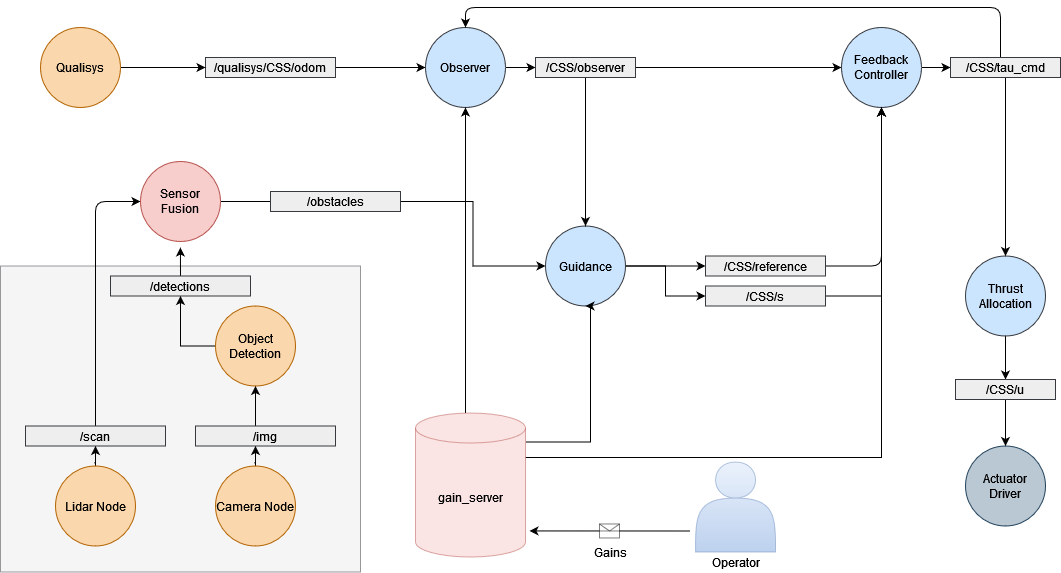
\includegraphics[width=\textwidth]{Images/ROS-topology(3).png}
    \caption{ROS-architecture of the CS Saucer.}
    \label{fig:ros-flow}
\end{figure}

\section{Vessel model}

\label{sec:modeling}

A mathematical model describing vessel dynamics is desirable in designing a control system and performing simulations. Starting from the equation of motion for a vessel at sea \citep{fossen_2021}, one can derive the necessary equations for the control model 

\begin{equation}
    \mathbf{M}_{RB}\dot{\boldsymbol{\nu}} + \mathbf{C}_{RB}\boldsymbol{\nu} + \mathbf{M}_A\dot{\boldsymbol{\nu}}_r + \mathbf{C}_A(\boldsymbol{\nu}_r)\boldsymbol{\nu}_r + \mathbf{D}(\nu_r)\nu_r + \mathbf{D}\boldsymbol{\nu}_r + \mathbf{g}(\boldsymbol{\eta}) = \tau_{ext},
\end{equation}

where:

\begin{itemize}
    \item $ \boldsymbol{\nu} = \big[ u \ v  \ r \big]^{\top}$ is the body-fixed velocities in surge, sway and yaw.
    \item $\boldsymbol{\nu}_r$ is the body-fixed velocities relative to local current in surge, sway and yaw
    \item $\mathbf{M}_{RB}$ and $\mathbf{M}_A$ is the vessel inertia matrix for mass and added mass
    \item $\mathbf{C}_{RB}$ and $\mathbf{C}_A(\nu_r)$ is the vessel Coriolis matrix for rigid body and added mass respectively. 
    \item $\mathbf{D}(\nu_r)$ is the nonlinear damping matrix
    \item $\mathbf{D}$ is the linear damping matrix
    \item $\mathbf{g}(\eta)$ is the hydro-static restoring matrix
    \item $\boldsymbol{\tau}_{ext} = \big[ X \ Y  \ N \big]^{\top}$ is the external forces acting in surge, sway and yaw
\end{itemize}

A model derivation was conducted by \citet{ueland} for his master thesis, which will be reused in this project. The following assumptions were made for the model: 

\begin{enumerate}
    \item Zero current in the MC-lab, $\nu_r = \nu$.
    \item The CSS is self-stabilizing by hydrostatic forces in heave, roll, and pitch. The rotations are considered small, so movements in surge, sway, and yaw are not affected by the configuration in pitch and roll. 
    \item No  hydrostatic restoring forces in surge, sway and yaw, $\mathbf{g}(\eta) = 0$.
    \item Constant frequencies, meaning that damping and added mass are also considered constant.
    \item The hull of the CSS is assumed to be completely symmetric.
\end{enumerate}

The resulting control design model is equivalent to the simplified model presented by \citet{fossen_2021}, which is a good representation of a 3DOF marine craft not affected by environmental forces, that is,

\begin{align*}
    \mathbf{\dot{\eta}} &= \mathbf{R(\psi)}\mathbf{\nu} \\
    \mathbf{M}\mathbf{\dot{\nu}} + (\mathbf{C} + \mathbf{D} + \mathbf{D}(\mathbf{\nu}))\nu &= \mathbf{\tau},
\end{align*}

where:

\begin{itemize}
    \item The inertia matrix $\mathbf{M}$
    \begin{equation}
    \mathbf{M} = \begin{bmatrix}9.51 & 0 & 0 \\ 0 & 9.51 & 0 \\ 0 & 0 & 0.116 \end{bmatrix}
    \end{equation}
    \item The Coriolis matrix $\mathbf{C}$
        \begin{equation}
    \mathbf{C} = \begin{bmatrix}0 & -9.51r & 0 \\  9.51r & 0 & 0  \\ 0 & 0 & 0 \end{bmatrix}
    \end{equation}
    \item The linear damping matrix $\mathbf{D}$
   \begin{equation}
    \mathbf{D} =  \begin{bmatrix}1.96 & 0 & 0 \\ 0 & 1.96 & 0 \\ 0 & 0 & 0.168 \end{bmatrix}
    \end{equation}
    \item The non-linear damping matrix $\mathbf{D(\nu)}$
    \begin{equation}
    \mathbf{D(\boldsymbol{\nu})} =  \begin{bmatrix}7.095|u| & 0 & 0 \\ 0 & 7.095|v| & 0 \\ 0 & 0 & 7.095|r| \end{bmatrix}
    \end{equation}
    \item The rotation matrix $R(\psi)$ 
    \begin{equation}
        \mathbf{R}(\psi) = \begin{bmatrix}\cos({\psi}) & -\sin{(\psi)} & 0 \\
        \sin{(\psi)} & \cos{(\psi)} & 0 \\ 0 & 0 & 1\end{bmatrix}
    \end{equation}
\end{itemize}

\section{Sensor integration}

A new top module was issued for the CSS as part of \citet{solheim-master} On top of it, two sensors were integrated along with tracking markers for the Qualisys motion capture system present in the MC-lab. The Qualisys system acts as a GPS for the vessel, providing the control system with measurements of the vessel's position and orientation. The markers are mounted on slender rods of varying heights along the circumference of the module. Then, the lidar is mounted in the center, directly above the CO of the CSS. The sensor is oriented so the $x_l$ and $y_l$ axis of the lidar align with the surge and sway directions, respectively. While the lidar provides a 360-degree scan, the interval of  $[-90^\circ, 90^\circ]$ is most interesting. Thus markers are mounted to cause as little interference as possible and still provide an accurate estimation of the vessel states. The same constraints apply to the placement of the camera. It requires an unobstructed view but can not interfere with the lidar in the critical area. Therefore it is mounted on a slender rod right behind the lidar with enough clearance to the lidar that it sees the environment clearly. The camera is tightly connected to the vessel heading, always pointing in the direction that is considered forward. Accordingly, it is mounted so that the $z_c$- and $x_c$-axis align with the surge and sway directions of the CSS.

\begin{figure}[ht]
     \centering
     \begin{subfigure}[b]{0.25\textwidth}
        \centering
        \begin{tikzpicture}
        \begin{scope}[scale=0.8]
        % place nodes
        \coordinate (a) at (0,0.5);% Change 1.5 to change the shape of the droplet
        \draw[semitransparent] (0,0) circle[radius=3cm]; % test of the radius size
        \draw[-latex] (0,0) -- (4, 0) node[below]{$\mathbf{Y}$};
        \draw[-latex] (0,0) -- (0, 4) node[left]{$\mathbf{X}$};
        \draw[fill=gray, semitransparent] (0,-2.45) circle[radius=5pt] node[left, xshift=-0.15cm] {\tiny Qualisys};;
        \draw[fill=gray, semitransparent] (2.45,0) circle[radius=5pt];
        \draw[fill=gray, semitransparent] (-2.05,1.2) circle[radius=5pt];
        \draw[-latex, dashed, red] (0,0) -- (2, 0) node[below]{$\mathbf{y_l}$};
        \draw[-latex, dashed, red] (0,0) -- (0, 2) node[left]{$\mathbf{x_l}$};
        \node [circle,draw, fill=gray, gray] (c) at (0,0) [minimum size=20pt] {$c$};
        \draw[gray, fill] (a) -- (tangent cs:node=c,point={(a)},solution=1) --
        (c.center) -- (tangent cs:node=c,point={(a)},solution=2) -- cycle;
        \draw[fill=black, semitransparent] (0, 0) circle [radius=8pt] node[left, xshift=-0.3cm] {\tiny LiDAR};
        \draw[-latex, dashed, blue] (0,-0.6) -- (2, -0.6) node[below]{$\mathbf{x_c}$};
        \draw[-latex, dashed, blue] (0,-0.6) -- (0, 1.4) node[left]{$\mathbf{z_c}$};
        \draw[fill=black] (-0.1, -0.5) rectangle(0.1, -0.7) node[left, yshift=-0.15cm, semitransparent] {\tiny Cam};
        \draw[fill=black] (0, -0.5) -- (-0.1, -0.45) -- (0.1, -0.45) -- (0, -0.5);
     \end{scope}
     \end{tikzpicture}
     \end{subfigure}
     \hfill
     \begin{subfigure}[b]{0.45\textwidth}
        \centering
        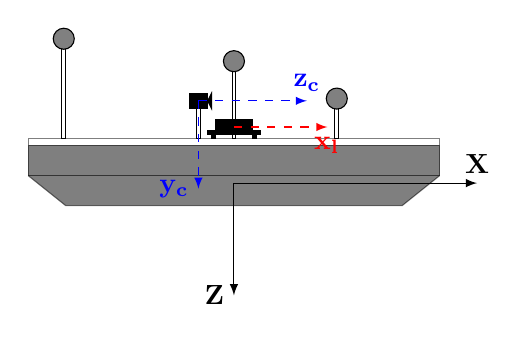
\begin{tikzpicture}
        \begin{scope}[scale=0.95]
        % place nodes
        \draw[semitransparent] (0, 0) rectangle (5.5, 0.1);
        \draw[fill=black, semitransparent] (0, 0) rectangle (5.5, -0.4);
        \draw[fill=black, semitransparent] (0, -0.4) -- (0.5, -0.8) -- (5, -0.8) -- (5.5, -0.4);
        \draw (2.725, 0.1) rectangle (2.775, 1);
        \draw[fill=gray] (2.75, 1.13) circle(4pt);
        \draw (4.1, 0.1) rectangle (4.15, 0.5);
        \draw[fill=gray] (4.125, 0.63) circle(4pt);
        \draw (0.45, 0.1) rectangle (0.5, 1.3);
        \draw[fill=gray] (0.475, 1.43) circle(4pt);
        \draw[fill=black] (2.45, 0.1) rectangle (2.5, 0.15);
        \draw[fill=black] (3, 0.1) rectangle (3.05, 0.15);
        \draw[fill=black] (2.40, 0.15) rectangle (3.1, 0.20);
        \draw[fill=black] (2.5, 0.15) rectangle (3, 0.35);
        \draw (2.25, 0.1) rectangle (2.30, 0.5);
        \draw[fill=black] (2.15, 0.5) rectangle (2.4, 0.7); 
        \draw[fill=black] (2.4, 0.6) -- (2.45, 0.7) -- (2.45, 0.5) -- (2.4, 0.6);
        \draw[-latex] (2.75, -0.5) -- (6, -0.5) node[above] {$\mathbf{X}$};
        \draw[-latex] (2.75, -0.5) -- (2.75, -2) node[left] {$\mathbf{Z}$};
        \draw[-latex, dashed, red] (2.75,0.25) -- (4, 0.25) node[below, xshift=-0.3]{$\mathbf{x_l}$};
        \draw[-latex, dashed, blue] (2.275, 0.6) -- (3.725, 0.6) node[above]{$\mathbf{z_c}$};
        \draw[-latex, dashed, blue] (2.275, 0.6) -- (2.275, -0.575) node[left]{$\mathbf{y_c}$};
        \end{scope}
    \end{tikzpicture}
     \end{subfigure}
        \caption{Sensor integration for the CS Saucer}
        \label{fig:sensor-suit}
\end{figure}

The open-source computer vision library OpenCV is utilized to establish an image stream between the camera and the object detection module. It provides a generic ROS camera driver that can be utilized with all Video4Linux (V4L2) compatible cameras and publishes the image stream to the ROS-topic \texttt{/cv\_camera/image\_raw}. In addition, Slamtec, the manufacturer of the RPLidar, provides a ROS driver for their hardware. The driver publishes the measured ranges to the topic \texttt{/scan}.